\chapter{Normalización de Flujos} \label{Metodologia:NormalizacionFlujos}

Tenemos a nuestra disposición las cuentas de fotones que corresponden a sus
magnitudes para las curvas de luz de Gaia, para las cuales el flujo reportado es
el promedio de todas las mediciones hechas en un transito, e Iturbide. Sin
embargo, estas cuentas crudas no son adecuadas para el ajuste de modelo con
PHOEBE; estas producen resultados no físicos cuando son utilizadas sin
tratamiento adicional. Para esto las magnitudes determinadas en la sección
anterior se convierten a flujos normalizados con la
\refequation{normFlujosEcuacion}. Esta transformación fue aplicada a todas las
curvas de luz recabadas (Gaia, ZTF, Iturbide) para poder trabajar con datos
consistentes al momento de desarrollar el modelo computacional en PHOEBE.

\begin{eqfloat}[!ht]
	\centering
	\begin{equation}
		f_p = 10^{-\frac{2}{5} \cdot (m_p - m_0)}
	\end{equation}
	\caption{Ecuación usada para obtener flujos para cada pasa banda $p$. Esta
		determina el flujo normalizado $f_p$ desde la magnitud reportada $m_p$
		utilizando una magnitud de referencia $m_0$.}
	\label{normFlujosEcuacion}
\end{eqfloat}

\section{Preservación de Color}

% TODO: figure out how to cite specific chapter of PHOEBE textbook (page 111) without having to create a bunch of citations for each section used
	% ideally would mention the chapters/pages used in a single citation
Gracias a las observaciones en varias pasa bandas tenemos información del color
del sistema, debido a la diferencia de magnitud. Sin embargo PHOEBE trabaja solo
con flujos, por lo cual la transformación descrita en la
\refthesissection{Metodologia:NormalizacionFlujos} fue necesaria. Para preservar el
color por diferencia de magnitud se determina un solo valor de $m_0$ con el cual
convertir las magnitudes; este $m_0$ corresponde a la magnitud en 0.25 de fase
del pasa bandas más tenue del sistema. PHOEBE tablas de coeficientes que
relacionan la temperatura efectiva del sistema binario con la diferencia de
flujos. \citeyearparen{phoebeScientificReference} 

En este trabajo se dividieron las curvas de luz de \atoObjId basado en su
fuente: las de Gaia ($G, G_{BP}, G_{RP}$), las de ZTF ($ZTF:G, ZTF:R$), y la de
Iturbide. Podemos determinar 2 diferentes colores del sistema, entre la
diferencia de color en Gaia y ZTF (como solo se observó a \atoObjId con un solo
filtro en Iturbide no contamos con datos de color). Para ZTF se tomó la
magnitud de $ZTF:G$. Las curvas de luz en fase se pueden ver en la
\reffigure{normFlujosCurvas}, donde se puede apreciar como preserva la
diferencia de magnitud vista en \reffigure{gaiaIturbideZtfPhaseFold}. El
código responsable de esta reducción se encuentra en
\href{https://github.com/KnightIV/UANL_MAPTA_Observaciones/blob/main/analisis/gaia/light_curves.ipynb}{\code{light\_curves.ipynb}}
para Gaia,
\href{https://github.com/KnightIV/UANL_MAPTA_Observaciones/blob/main/analisis/ztf/light-curve-processing.ipynb}{\code{light-curve-processing.ipynb}}
para ZTF, y
\href{https://github.com/KnightIV/UANL_MAPTA_Observaciones/blob/main/analisis/iturbide/iraf/qphot_timeseries_analysis.ipynb}{\code{qphot\_timeseries\_analysis.ipynb}}
para Iturbide.

\begin{figure}[!ht]
	\centering
	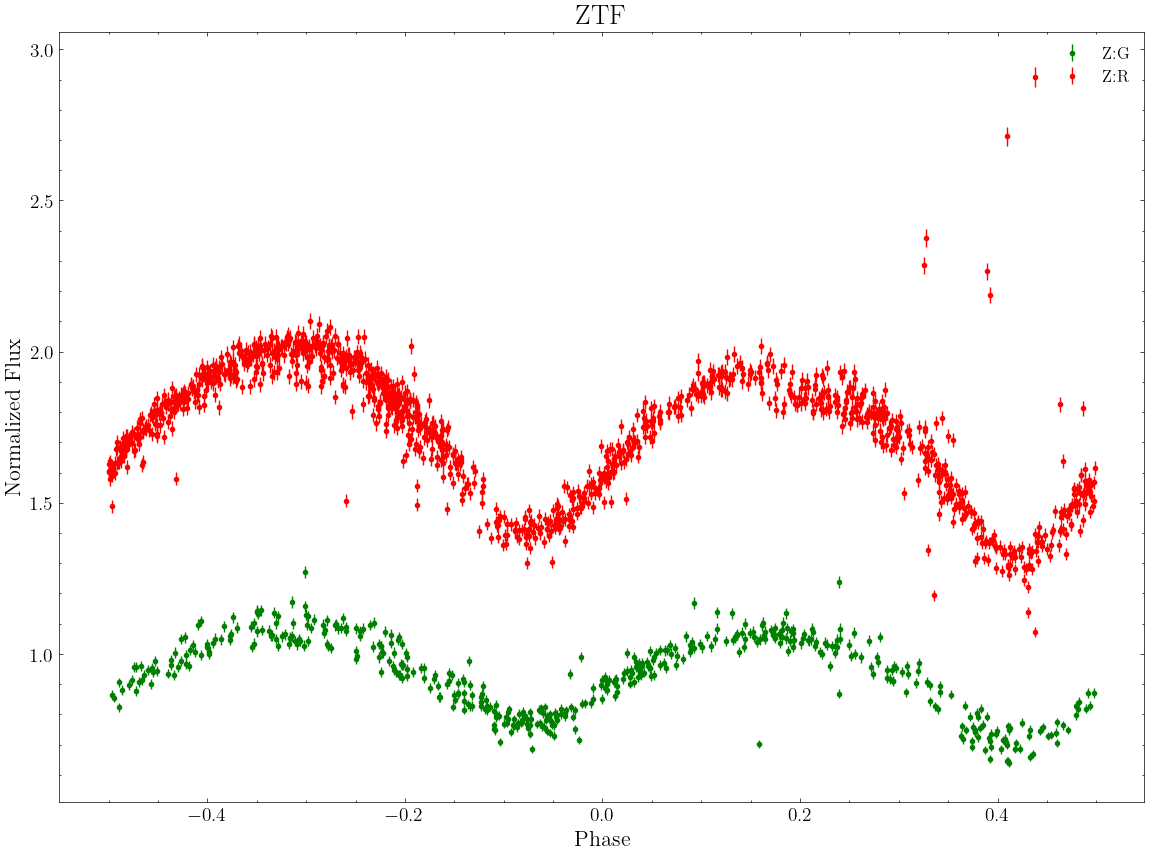
\includegraphics[scale=0.3]{Metodologia/Secciones/NormalizacionFlujos/Figures/ZTF Normalized Flux.png}
	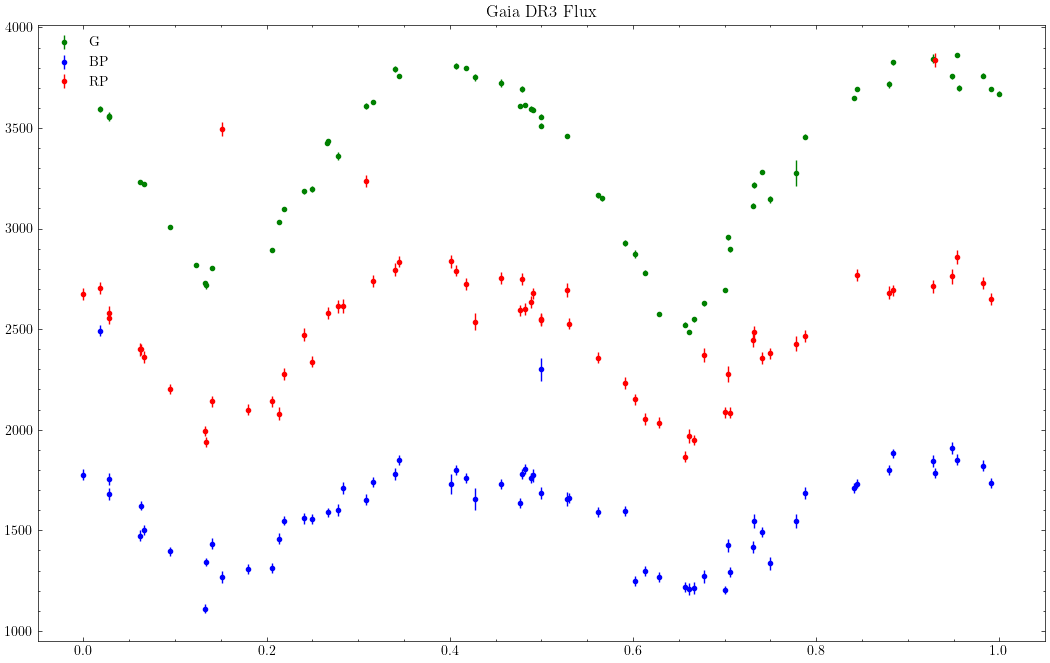
\includegraphics[scale=0.3]{Metodologia/Secciones/NormalizacionFlujos/Figures/GDR3 Flux.png}
	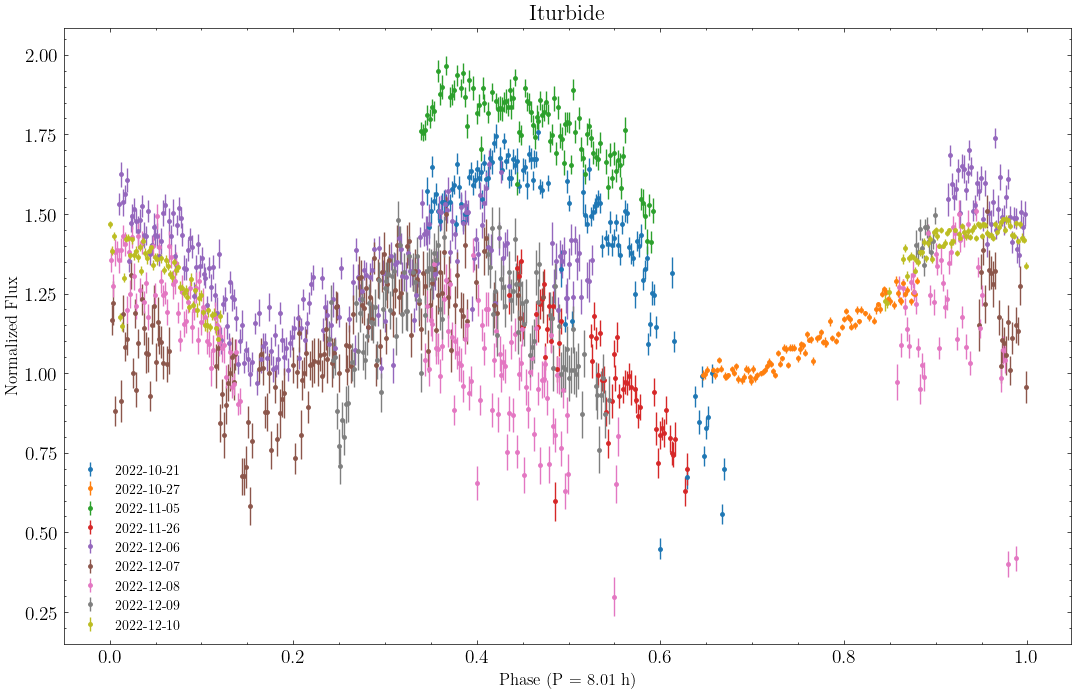
\includegraphics[scale=0.4]{Metodologia/Secciones/NormalizacionFlujos/Figures/Iturbide Normalized Flux.png}

	\caption{Flujo en fase de cada curva de luz utilizada. El catálogo de Gaia
		DR3 ya tiene reportado el flujo del sistema, por lo cual este se utilizó
		para el modelo en vez de obtener un flujo normalizado partiendo de las
		magnitudes.}
	\label{normFlujosCurvas}
\end{figure}